\chapter{State of the Art}
\label{ch:state-of-art}

This chapter reviews the current state of knowledge across the domains that intersect in this thesis: the \gls{iomt} ecosystem and its security challenges, \gls{ids} approaches with emphasis on \gls{ml}-based methods, the benchmark datasets available for network intrusion detection research, and the preprocessing tools that transform raw network traffic into representations suitable for model training. The chapter concludes by identifying the specific gaps that this thesis aims to address.

% ══════════════════════════════════════════════════════════════════════════════
\section{The Internet of Medical Things}
\label{sec:iomt}

\subsection{Definition and Evolution}
\label{subsec:iomt-def}

The \gls{iomt} refers to the interconnected infrastructure of medical devices, software applications, and health systems that communicate over networks to enable healthcare delivery and monitoring~\cite{dimitrov2016medical}. Unlike general-purpose \gls{iot} deployments, \gls{iomt} environments are characterized by stringent requirements on reliability, latency, and data confidentiality, driven by their direct impact on patient safety~\cite{domenech2024ensuring}.

The \gls{iomt} ecosystem encompasses a broad spectrum of devices, including but not limited to: wearable health monitors (electrocardiographs, pulse oximeters), smart infusion pumps, connected imaging systems, remote patient monitoring platforms, and hospital asset tracking systems. These devices typically communicate using lightweight protocols such as \gls{mqtt} and \gls{coap}, which are optimized for resource-constrained environments but were not originally designed with comprehensive security mechanisms~\cite{domenech2025preventive}.

\subsection{Security Challenges}
\label{subsec:iomt-security}

The convergence of clinical operations with network connectivity exposes \gls{iomt} environments to a wide range of cyber threats. The \gls{enisa} reported a significant increase in cyberattacks targeting the health sector between 2021 and 2023, with hospitals, healthcare providers, and medical device manufacturers among the most affected entities~\cite{enisa2023health}.

Several characteristics of \gls{iomt} environments amplify the security challenge:

\begin{itemize}
    \item \textbf{Resource constraints.} Many medical devices operate with limited computational resources, restricting the deployment of conventional security mechanisms such as encryption or deep packet inspection at the device level.

    \item \textbf{Heterogeneous protocols.} The coexistence of multiple communication protocols (Wi-Fi, \gls{ble}, \gls{mqtt}, \gls{coap}, ZigBee) within a single clinical environment creates a complex attack surface with diverse vulnerability profiles~\cite{dadkhah2024ciciomt}.

    \item \textbf{Legacy systems.} Healthcare environments frequently operate medical devices with long lifecycles, many of which lack support for modern security patches or firmware updates.

    \item \textbf{Patient safety implications.} Unlike many other \gls{iot} domains, compromised \gls{iomt} devices---particularly active devices such as infusion pumps or ventilators---can directly endanger patient health, elevating the consequences of successful attacks beyond data theft to potential physical harm~\cite{domenech2024ensuring}.
\end{itemize}

The attack landscape in \gls{iomt} environments includes reconnaissance activities, \gls{arp} spoofing, man-in-the-middle attacks, various forms of \gls{dos} and \gls{ddos} attacks, data injection, and protocol-specific attacks targeting \gls{mqtt} or \gls{coap} communications~\cite{leon2025miotta}. This diversity of attack vectors necessitates detection systems capable of identifying a wide spectrum of malicious behaviors.

% ══════════════════════════════════════════════════════════════════════════════
\section{Intrusion Detection Systems}
\label{sec:ids}

\subsection{Taxonomy}
\label{subsec:ids-taxonomy}

An \gls{ids} is a security mechanism designed to monitor network traffic or system activities and identify potential security violations. The literature typically classifies \gls{ids} along two orthogonal dimensions~\cite{khraisat2019survey}:

\paragraph{By data source:}
\begin{itemize}
    \item \textbf{\Gls{nids}:} Monitors network traffic at strategic points, analyzing packet headers and payloads to detect suspicious patterns. This approach is particularly suitable for \gls{iomt} environments where installing host-based agents on resource-constrained devices is impractical.

    \item \textbf{\Gls{hids}:} Operates on individual hosts, monitoring system calls, file integrity, and local network connections. While effective for servers and workstations, its applicability to \gls{iomt} devices is limited by their computational constraints.
\end{itemize}

\paragraph{By detection method:}
\begin{itemize}
    \item \textbf{\Gls{sids}:} Detects intrusions by matching observed patterns against a database of known attack signatures. This approach achieves high precision for known threats but is inherently unable to detect novel or zero-day attacks.

    \item \textbf{\Gls{aids}:} Establishes a baseline model of normal system behavior and flags deviations as potential intrusions. This approach can detect previously unseen attacks but is susceptible to higher false positive rates, particularly during the initial profiling phase.
\end{itemize}

For \gls{iomt} environments, the combination of network-based deployment and anomaly-based detection is generally considered the most viable approach, as it does not require modifications to the medical devices themselves and can potentially detect novel threats~\cite{domenech2024ensuring, weber2023attack}.

\subsection{Machine Learning for Intrusion Detection}
\label{subsec:ml-ids}

The application of \gls{ml} techniques to intrusion detection has attracted substantial research attention, driven by the ability of learning algorithms to automatically extract discriminative patterns from network traffic data~\cite{ahmad2021network, sarker2021ml}.

\paragraph{Traditional \gls{ml} approaches.} Algorithms such as \gls{rf}, \gls{dt}, \gls{svm}, \gls{knn}, and \gls{xgb} have been widely applied to network intrusion detection, typically operating on engineered feature vectors derived from network flows or traffic windows. These methods benefit from relatively low computational requirements and interpretability, making them suitable for deployment in resource-aware environments~\cite{heidari2023iot}.

\paragraph{\Gls{dl} approaches.} Neural network architectures, including \glspl{cnn}, \glspl{rnn}, and hybrid models, have demonstrated the ability to learn hierarchical feature representations directly from network data. Recent work has explored \gls{tsc} models that process sequences of packets or traffic windows, capturing temporal dynamics that may be indicative of ongoing attacks~\cite{lopez2025nprint}.

\paragraph{Challenges.} Despite the promising results reported in the literature, the practical deployment of \gls{ml}-based \gls{ids} in \gls{iomt} environments faces several persistent challenges: (i)~the lack of representative training data that captures the diversity of real-world attack scenarios, (ii)~the difficulty of achieving generalization across different network environments, and (iii)~the trade-off between detection accuracy and computational efficiency~\cite{domenech2025evaluating}.

% ══════════════════════════════════════════════════════════════════════════════
\section{Benchmark Datasets for IoMT/IoT Intrusion Detection}
\label{sec:datasets}

The quality and characteristics of the training data fundamentally determine the performance ceiling of any \gls{ml}-based \gls{ids}. This section reviews the two \gls{iomt}-specific datasets used for training and the real hospital network dataset used for deployment-environment evaluation, alongside other relevant benchmarks.

\subsection{CICIoMT2024}
\label{subsec:ciciomt2024}

The CICIoMT2024 dataset~\cite{dadkhah2024ciciomt}, developed by the Canadian Institute for Cybersecurity (\gls{cic}), is specifically designed for multi-protocol security assessment in \gls{iomt} environments. It captures network traffic from 40 real and emulated medical devices communicating over five protocols: Wi-Fi, \gls{mqtt}, \gls{ble}, ZigBee, and a combined multi-protocol scenario.

The dataset encompasses 18 distinct attack types organized into broad categories including \gls{ddos}, \gls{dos}, reconnaissance, spoofing, and \gls{mqtt}-specific attacks. The original dataset provides 45 features extracted using the CIC's internal preprocessing tools, with features computed at both flow and window levels. The dataset includes approximately 54 million records distributed across training and testing partitions.

Key characteristics relevant to this thesis include the multi-protocol coverage, the diversity of attack types, and the availability of raw \gls{pcap} files that enable reprocessing with alternative feature extraction tools.

\subsection{IoMT-TrafficData}
\label{subsec:iomt-trafficdata}

The IoMT-TrafficData dataset~\cite{areia2024iomt} provides network traffic captures from an \gls{iomt} testbed simulating a hospital environment with both real and simulated medical devices. The dataset captures six categories of attacks: \gls{arp} spoofing, data malformation, \gls{dos}, \gls{ddos}, reconnaissance, and their combinations.

In its original form, the dataset provides 101 features extracted using Zeek~\cite{zeek} at the flow level. The features encompass connection metadata, flow-level statistics, packet size distributions, \gls{tcp} flag counts, inter-arrival times, and directional traffic metrics. The Zeek-based extraction methodology differs fundamentally from the window-based approach used by the CIC datasets, creating a structural incompatibility that complicates direct integration.

This dataset is particularly valuable for its focus on IoMT-specific attack scenarios that complement the CICIoMT2024 coverage, especially in the areas of data malformation and combined attack patterns.

\subsection{HospNet26}
\label{subsec:hospnet26}

The HospNet26 dataset~\cite{hospnet26} is a real-world hospital network traffic capture collected from a production clinical network during normal operation in 2026. Unlike the two testbed datasets described above, it contains exclusively legitimate traffic---no injected attacks are present---making it the first publicly available real-world reference dataset for network security research in a healthcare setting~\cite{domenech2026robust}.

The dataset is organized into four temporal segments (Friday, Weekend, Monday, and Tuesday--Friday), totalling 1,265,240 windows after processing with MIOTTA-NPT in combined mode using the same 100-packet window configuration as the training datasets. All 58 MIOTTA features extracted from HospNet26 are shared with the training feature space, enabling direct model inference without any feature adaptation.

In this thesis, HospNet26 serves as a \textbf{real-world deployment probe}: the trained \gls{ids} models are applied to its traffic without retraining or adaptation. Since all traffic is presumed benign, the fraction of windows classified as \texttt{Benign} (the benign prediction rate $r_B$) provides a quantitative measure of model specificity under genuine clinical network conditions.

\subsection{Other Relevant Datasets}
\label{subsec:other-datasets}

Several other datasets have contributed to the \gls{iomt} and \gls{iot} intrusion detection research landscape:

\begin{itemize}
    \item \textbf{WUSTL-EHMS}~\cite{hady2020ids}: A dataset from a simulated electronic health monitoring system, incorporating both network and biometric data with 34 flow-level features.

    \item \textbf{IoT-Healthcare}~\cite{hussain2021framework}: A dataset using real and simulated medical devices with 50 packet-level features, accompanied by publicly available preprocessing tools.

    \item \textbf{CICIoT2023}~\cite{neto2023ciciot2023}: A large-scale general \gls{iot} dataset from the \gls{cic} capturing network traffic from 105 \gls{iot} devices across 33 attack types. While not used in the integration phase of this thesis, it represents an important benchmark in the broader \gls{iot} intrusion detection literature.
\end{itemize}

\subsection{Comparative Analysis of Selected Datasets}
\label{subsec:dataset-comparison}

Table~\ref{tab:dataset-comparison} summarizes the key characteristics of the three datasets selected for this thesis.

\begin{table}[htbp]
\centering
\caption{Comparative summary of the datasets used in this thesis.}
\label{tab:dataset-comparison}
\small
\begin{tabularx}{\textwidth}{@{}l X X X@{}}
\toprule
\textbf{Characteristic} & \textbf{CICIoMT2024} & \textbf{IoMT-TrafficData} & \textbf{HospNet26} \\
\midrule
Role & Training / testing & Training / testing & Generalization probe \\
Domain & IoMT testbed & IoMT testbed & Real hospital network \\
Year & 2024 & 2024 & 2026 \\
Devices & 40 (real + emulated) & Real + simulated & Production clinical \\
Protocols & Wi-Fi, MQTT, BLE, ZigBee & MQTT, CoAP & Multiple \\
Attack types & 18 & 6 categories & None (benign only) \\
Original features & 45 & 101 (Zeek) & N/A \\
Extraction tool & CIC internal & Zeek & MIOTTA-NPT \\
Extraction level & Flow + Window & Flow & Window (combined) \\
PCAP available & Yes & Yes & Yes \\
\bottomrule
\end{tabularx}
\end{table}

A critical observation emerges from the two training datasets: CICIoMT2024 and IoMT-TrafficData employ structurally incompatible feature extraction methodologies---CICFlowMeter-based flow statistics versus Zeek-derived per-connection records, respectively. This structural mismatch makes direct concatenation or cross-dataset comparison infeasible without returning to the raw \gls{pcap} captures. HospNet26, by contrast, is already available in MIOTTA-NPT combined-mode format, sharing the same 58-feature representation as the reprocessed training datasets and therefore requiring no feature adaptation for inference. This feature heterogeneity between the two training sources constitutes the primary technical challenge addressed by this thesis.

% ══════════════════════════════════════════════════════════════════════════════
\section{Network Traffic Preprocessing and Feature Extraction}
\label{sec:preprocessing}

The transformation of raw network traffic into structured representations suitable for \gls{ml} models is a critical step in the \gls{ids} pipeline. The choice of preprocessing methodology directly influences the quality and expressiveness of the resulting features, and consequently, the upper bound on model performance~\cite{leon2025miotta}.

\subsection{Feature Extraction Approaches}
\label{subsec:extraction-approaches}

Network traffic feature extraction can be categorized along several dimensions:

\paragraph{Granularity.}
\begin{itemize}
    \item \textbf{Packet-level}: Each individual packet generates one feature vector, capturing attributes such as header fields, payload size, and protocol flags. This provides the finest granularity but results in very large datasets and may not capture temporal relationships between packets.

    \item \textbf{Flow-level}: Packets sharing the same 5-tuple (source/destination IP, source/destination port, protocol) are aggregated into flows, and statistical features are computed over the entire flow. Tools such as CICFlowMeter~\cite{cicflowmeter} and Zeek~\cite{zeek} operate at this level. This approach captures connection-level behavior but loses intra-flow temporal dynamics.

    \item \textbf{Window-level}: Packets are grouped into fixed-size windows (e.g., every $N$ packets), and features are computed over each window. This provides a balance between granularity and context, capturing short-term traffic patterns while maintaining a manageable dataset size.

    \item \textbf{Combined}: Flow identification is performed within each window, yielding per-flow statistics contextualized within a temporal window. This approach, adopted by MIOTTA-NPT in its \textit{combined} mode, captures both flow-level semantics and temporal windowing.
\end{itemize}

\paragraph{Feature engineering philosophy.}
\begin{itemize}
    \item \textbf{Statistical features}: Hand-crafted features such as packet counts, byte totals, header lengths, flag distributions, and inter-arrival time statistics. These features encode domain knowledge about what aspects of network traffic are informative for intrusion detection.

    \item \textbf{Raw representations}: Approaches such as nPrint~\cite{holland2021nprint} that encode packets as binary vectors, delegating feature discovery to the \gls{ml} model. While potentially more expressive, this approach requires significantly more computational resources for model training.
\end{itemize}

\subsection{MIOTTA-NPT: Network Preprocessing Tool}
\label{subsec:miotta-npt}

\begin{figure}[htbp]
\centering
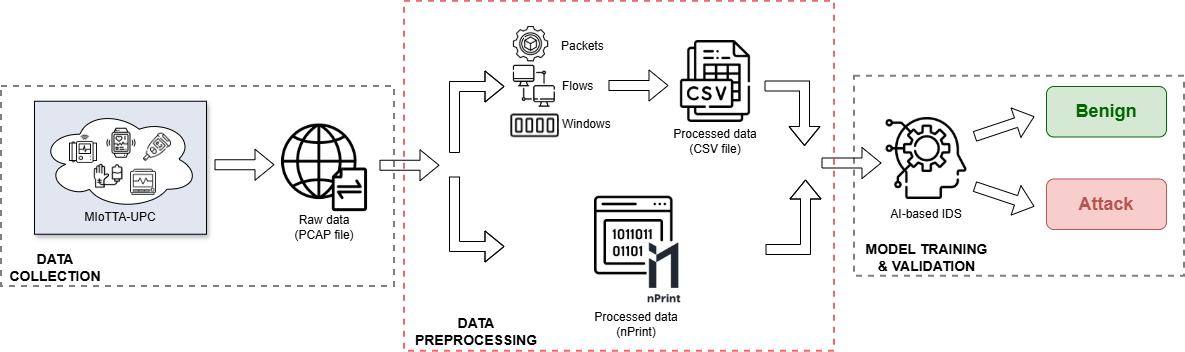
\includegraphics[width=0.85\textwidth]{miotta_npt_workflow.png}
\caption{MIOTTA-NPT tool workflow: from raw \gls{pcap} captures to structured feature datasets. The tool supports four extraction modes (packet, flow, window, combined) and two output formats (CSV, nPrint). Source:~\cite{miotta_npt_github}.}
\label{fig:miotta-workflow}
\end{figure}

The MIOTTA-NPT (Network Preprocessing Tool)~\cite{leon2025miotta, miotta_npt_github} is a configurable, open-source tool developed by the research group at UPC for transforming \gls{pcap} files into structured datasets. It occupies a central role in this thesis, as it provides the mechanism through which feature heterogeneity across datasets is resolved.

\paragraph{Architecture and modes.} The tool accepts \gls{pcap} files as input and supports two primary output formats: (i) CSV with statistical features, and (ii) nPrint binary representations. For the CSV output, four aggregation modes are available---packet, flow, window, and combined---allowing researchers to configure the extraction granularity according to their experimental needs.

\paragraph{Feature set.} In its combined mode (flow + window), the tool extracts up to 103 configurable features organized into three categories: 25 packet-level attributes, 42 flow-level statistics, and 36 window-level aggregations. These features capture a comprehensive range of traffic characteristics, including:

\begin{itemize}
    \item Connection metadata (IP addresses, ports, protocols)
    \item Packet size statistics (min, max, mean, standard deviation)
    \item Directional metrics (forward/backward packet counts, byte totals, rates)
    \item \gls{tcp} flag distributions
    \item \gls{iat} statistics
    \item Flow dynamics (covariance, variance ratio, weight, magnitude)
\end{itemize}

\paragraph{Significance for integration.} The key advantage of MIOTTA-NPT for dataset integration is its ability to process raw \gls{pcap} captures from any dataset through the same extraction pipeline, yielding identical feature spaces regardless of the source dataset. By reprocessing the \gls{pcap} files of CICIoMT2024 and IoMT-TrafficData through MIOTTA-NPT with identical configuration parameters (combined mode, window size of 100 packets), the fundamental challenge of feature heterogeneity is resolved at the source rather than through post-hoc feature mapping or engineering.

\paragraph{Comparison with existing tools.} Table~\ref{tab:tool-comparison} positions MIOTTA-NPT relative to other preprocessing tools in the literature.

\begin{table}[htbp]
\centering
\caption{Comparison of network traffic preprocessing tools~\cite{leon2025miotta}.}
\label{tab:tool-comparison}
\small
\begin{tabularx}{\textwidth}{@{}l c X p{2.2cm} c c@{}}
\toprule
\textbf{Tool} & \textbf{Year} & \textbf{Extraction Level} & \textbf{Format} & \textbf{Config.} & \textbf{\# Feat.} \\
\midrule
CICFlowMeter~\cite{cicflowmeter} & 2016 & Flow & CSV & No & 76 \\
WUSTL-EHMS~\cite{hady2020ids} & 2020 & Flow & CSV & No & 34 \\
IoT-Healthcare~\cite{hussain2021framework} & 2021 & Packet & CSV & No & 50 \\
CICIoT2023~\cite{neto2023ciciot2023} & 2023 & Flow + Window & CSV & No & 47 \\
CICIoMT2024~\cite{dadkhah2024ciciomt} & 2024 & Flow + Window & CSV & No & 45 \\
IoMT-TrafficData~\cite{areia2024iomt} & 2024 & Flow + Packet & CSV & No & 64 \\
\textbf{MIOTTA-NPT}~\cite{leon2025miotta} & \textbf{2025} & \textbf{All levels} & \textbf{CSV, nPrint} & \textbf{Yes} & \textbf{103} \\
\bottomrule
\end{tabularx}
\end{table}

% ══════════════════════════════════════════════════════════════════════════════
\section{Dataset Integration in Cybersecurity Research}
\label{sec:integration}

\subsection{The Challenge of Multi-Dataset Integration}
\label{subsec:integration-challenge}

The integration of multiple cybersecurity datasets is a recognized challenge in the research community, yet it remains underexplored. Most studies in \gls{ids} research rely on single datasets for training and evaluation, which limits the generalizability of the resulting models~\cite{domenech2025evaluating}. A comprehensive dataset-centric evaluation of federated \gls{ids} models across three IoT/IIoT datasets demonstrated that cross-dataset testing exposes substantial performance degradation---up to 30 percentage-point macro-F1 loss---when models trained on one dataset face unseen environments~\cite{abouhouran2025federated}. This finding empirically validates the necessity of multi-dataset integration for building robust detection systems.

The primary barriers to multi-dataset integration include:

\begin{enumerate}
    \item \textbf{Feature space mismatch}: Datasets extracted with different tools produce different feature sets, making direct concatenation impossible without feature engineering or re-extraction.

    \item \textbf{Semantic differences}: Even features with similar names may carry different semantics depending on the extraction methodology. For example, a ``flow duration'' computed by Zeek follows different aggregation rules than one computed by CICFlowMeter. Recent work on unified benchmarking formats has shown that such inconsistencies, together with data collection errors and duplication artifacts, are pervasive across popular \gls{nids} datasets~\cite{noblet2025nxcap}.

    \item \textbf{Label incompatibility}: Attack taxonomies and labeling conventions vary across datasets, with different granularity levels and naming schemes. Research on federated \gls{ids} has addressed this through harmonization to common family-level schemas, demonstrating that combined multi-dataset training with harmonized labels substantially restores cross-domain transfer performance~\cite{abouhouran2025federated}.

    \item \textbf{Distribution shifts}: Datasets captured in different network environments exhibit different baseline traffic distributions, which can confound model training if not properly addressed.
\end{enumerate}

\subsection{Approaches to Dataset Integration}
\label{subsec:integration-approaches}

The literature identifies several approaches to multi-dataset integration, ranging from general-purpose methodologies to domain-specific solutions:

\paragraph{General-purpose data unification.} Ali et al.~\cite{ali2015gudm} proposed the Global Unified Data Model (GUDM), a domain-independent framework for combining diverse data sources into unified datasets for learning and reasoning. Their approach employs a sequential pipeline of preprocessing methods (missing value handling, intrinsic relationship discovery, dataset reduction) followed by data modeling methods (priority-based attribute resolution, unified schema definition). A key contribution is the \textit{expert-centric priority-based} approach for resolving overlapping attributes---when multiple datasets contain semantically similar features, domain expert priorities determine which representation is preserved in the unified dataset. While developed for healthcare data, the underlying principles of systematic preprocessing, attribute conflict resolution, and unified schema generation are directly applicable to cybersecurity dataset integration.

\paragraph{PCAP-based re-extraction.} The most methodologically rigorous approach to achieving feature space unification is to reprocess raw network captures through a common extraction tool, yielding identical feature spaces by construction. Khan et al.~\cite{khan2024umnids} demonstrated this approach with the Unified Multimodal NIDS (UM-NIDS) dataset, which integrates four well-established datasets (CIC-IDS 2017, CIC-IoT 2023, UNSW-NB15, and CIC-DDoS 2019) by processing their raw \gls{pcap} files through a standardized three-stage pipeline that extracts flow-level features, packet payload information, and time-window-based contextual features. The resulting unified dataset enables cross-dataset validation and supports extensibility through the addition of new \gls{pcap} sources processed with the same tool. Complementarily, Noblet et al.~\cite{noblet2025nxcap} proposed Nxcap, a unified flow-oriented capture format for \gls{nids} benchmarking that bridges raw \gls{pcap} files and flow-level statistics. Their advanced deduplication engine revealed significant quality issues in established datasets, underscoring the importance of standardized processing pipelines that integrate data quality verification.

\paragraph{Feature-level semantic integration.} An alternative approach maps features from heterogeneous feature spaces into a common representation by identifying semantically equivalent features across datasets. This approach preserves the original feature extraction but requires careful validation that the mapped features are genuinely comparable. It is most suitable when the constituent datasets have been extracted using tools with similar underlying methodologies.

\paragraph{Federated label harmonization.} In distributed learning settings, recent work has demonstrated the effectiveness of harmonizing labels to a common family-level schema while aligning features to the intersection set across datasets~\cite{abouhouran2025federated}. Combined multi-dataset federation with harmonized labels yields approximately 90\% macro-F1 across datasets, significantly outperforming models trained on single datasets when evaluated cross-domain.

\subsection{Positioning of This Thesis}
\label{subsec:integration-positioning}

This thesis adopts a \textbf{hybrid strategy} that combines the strengths of the approaches described above. Following the PCAP-based re-extraction methodology validated by Khan et al.~\cite{khan2024umnids}, all constituent datasets are reprocessed through MIOTTA-NPT with identical configuration parameters, resolving feature heterogeneity at the source. The label harmonization follows a multi-level scheme informed by the family-level approach demonstrated in federated settings~\cite{abouhouran2025federated}, while extending it with fine-grained labels that preserve the original attack type information. The data quality assurance pipeline incorporates the preprocessing principles advocated by Ali et al.~\cite{ali2015gudm} and the deduplication awareness highlighted by Noblet et al.~\cite{noblet2025nxcap}. Finally, provenance tracking enables the cross-domain evaluation strategies whose importance has been empirically established in the recent literature~\cite{abouhouran2025federated, domenech2025evaluating}.

% ══════════════════════════════════════════════════════════════════════════════
\section{Chapter Summary and Identified Gaps}
\label{sec:gaps}

This review of the state of the art reveals the following key findings and gaps:

\begin{enumerate}
    \item \textbf{Growing threat landscape}: The \gls{iomt} domain faces an expanding array of cyber threats, with attacks increasing in both frequency and sophistication, underscoring the need for effective automated detection mechanisms.

    \item \textbf{Dataset limitations}: While several valuable benchmark datasets exist, each captures only a partial view of the threat landscape. No single dataset provides comprehensive coverage of the protocols, attack types, and device behaviors encountered in real-world \gls{iomt} deployments.

    \item \textbf{Feature heterogeneity barrier}: The use of different feature extraction tools and methodologies across datasets creates structural incompatibilities that have, to date, prevented systematic multi-dataset integration in the \gls{iomt} domain.

    \item \textbf{MIOTTA-NPT as enabler}: The availability of MIOTTA-NPT provides, for the first time, a configurable and open-source tool capable of processing raw captures from multiple datasets through a unified pipeline, resolving the feature heterogeneity barrier.

    \item \textbf{Lack of unified datasets}: No prior work has systematically integrated multiple \gls{iomt}/\gls{iot} datasets into a single, unified, \gls{ml}-ready dataset with harmonized labels and controlled provenance tracking.
\end{enumerate}

This thesis directly addresses gaps 3, 4, and 5 by leveraging MIOTTA-NPT as the foundation for a comprehensive dataset integration methodology, the design and execution of which are presented in the following chapters.
